\section{近似解的评价}
\label{sec:opt-approximate}

前四节讨论的是精确的解。实际计算几乎从不交出精确解：迭代在有限步后停止，浮点运算带来舍入。这就需要回答：拿到一个近似解，怎样说清它好到什么程度？我们会看到，“好”有几种不同的含义，它们回答不同的问题，只在一定条件下可以换算。

\paragraph{算法交出什么}
后面各章的方法都产生一列点。全卷用带括号的上标表示迭代步：$\bm{x}^{(t)}$是第$t$步的点，$t=0,1,\ldots,T$，$T$是总步数。括号把迭代编号与幂区分开，元素下标仍写在下面，如$x_i^{(t)}$。多数方法每一步沿某个方向走一段：
\begin{equation}
 \bm{x}^{(t+1)}=\bm{x}^{(t)}+\alpha^{(t)}\bm{d}^{(t)},
 \label{eq:opt-iteration}
\end{equation}
其中$\bm{d}^{(t)}$是方向，$\alpha^{(t)}>0$是步长。当前点的梯度和Hessian简记为$\bm{g}^{(t)}=\nabla f(\bm{x}^{(t)})$与$\bm{H}^{(t)}=\nabla^2f(\bm{x}^{(t)})$。

算法最后报告的点记为$\hat{\bm{x}}$。本节不关心它怎样得到，只关心怎样评价。要注意$\hat{\bm{x}}$与$\bm{x}^\star$的区别：前者是算法的输出，手里实实在在有；后者是问题的解，我们通常不知道。

\paragraph{目标差}
最直接的指标是目标差
\begin{equation}
 e_f(\hat{\bm{x}})=f(\hat{\bm{x}})-f^\star.
 \label{eq:opt-objective-gap}
\end{equation}
它回答“这个结果比最好的结果差多少”。可行点的目标差非负；若$\hat{\bm{x}}$可行且$e_f(\hat{\bm{x}})\leq\varepsilon$，就称它为$\varepsilon$最优解（$\varepsilon$-optimal solution）。

目标差的麻烦在于$f^\star$通常未知。但只要有一个下界$\ell\leq f^\star$，就有可以计算的上界$e_f(\hat{\bm{x}})\leq f(\hat{\bm{x}})-\ell$。资源分配中，“两条约束相加”给出了下界$\ell=-10$，它不依赖于解出$(2,2)$。对可行点$\hat{\bm{x}}=(1.5,2)$，利润是$8.5$，因此
\[
 f(\hat{\bm{x}})-\ell=-8.5-(-10)=1.5.
\]
这正是上下界夹逼的用处：不知道解在哪里，也能确认当前结果至多差$1.5$。这样的下界怎样系统地构造，是第~\ref{chap:duality}章的主题。

\paragraph{解距离}
第二个指标问位置差多远。设最优解集合$\bm{S}$非空，定义到解集的距离
\begin{equation}
 e_d(\hat{\bm{x}})=\operatorname{dist}(\hat{\bm{x}},\bm{S})=\inf_{\bm{x}\in\bm{S}}\lVert\hat{\bm{x}}-\bm{x}\rVert_2.
 \label{eq:opt-solution-distance}
\end{equation}
解唯一时，它就是$\lVert\hat{\bm{x}}-\bm{x}^\star\rVert_2$。

解不唯一时要注意参照对象。实例~\eqref{eq:opt-ridge-instance}取$\gamma=0$，点$(11,-9)$在直线$x_1+x_2=2$上，它本身就是最优解，到解集的距离为$0$。若心里的“正确系数”是$(1,1)$，两者却相距$\lVert(10,-10)\rVert_2\approx14.1$。把解距离写成到某一个解的距离，就在问题没有提供信息的地方提了要求。

\paragraph{梯度大小}
前两个指标都含有未知量，第三个可以直接算：
\begin{equation}
 e_g(\hat{\bm{x}})=\lVert\nabla f(\hat{\bm{x}})\rVert_2.
 \label{eq:opt-gradient-size}
\end{equation}
由第~\ref{sec:opt-optimality}节，无约束时局部最优解的梯度为零，所以梯度大小可以作为一种缺口的度量。满足$e_g(\hat{\bm{x}})\leq\varepsilon$的点称为$\varepsilon$驻点（$\varepsilon$-stationary point）。

梯度小却不等于接近解。图~\ref{fig:opt-flat-gradient}(a)比较$f_1(x)=0.005x^2$与$f_2(x)=0.5x^2$，两者的最小点都是$0$。在$x=10$处$f_1'=0.1$，在$x=0.1$处$f_2'=0.1$，梯度一样大。前者的目标差是$0.5$，距离是$10$；后者分别是$0.005$和$0.1$。原因在曲率：$f_1$的二阶导数只有$0.01$，地形太平，坡度很小时离谷底仍然很远。

\begin{BookInlineFigure}
  \centering
  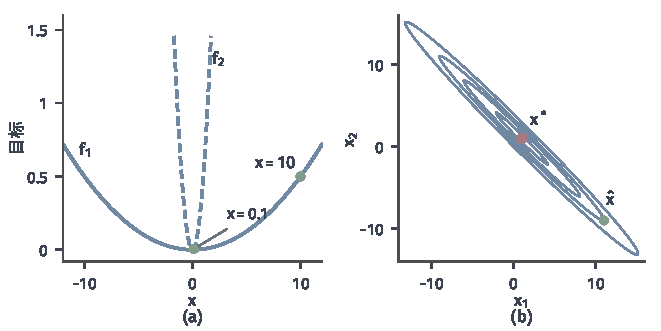
\includegraphics[width=112mm]{figures/05-optimization/01-linear-programming/matplotlib/opt-flat-gradient/figure.pdf}
  \caption{小梯度与小误差。(a)平坦的$f_1(x)=0.005x^2$（实线）在$x=10$处与陡峭的$f_2(x)=0.5x^2$（虚线）在$x=0.1$处导数都是$0.1$，目标差和距离却相差约两个量级。(b)拟合实例取$\gamma=0.01$，蓝线是目标差等于$0.1,0.5,1,2$的等高线，沿$(1,-1)$方向被拉得极长。绿点$\hat{\bm{x}}=(11,-9)$的梯度大小约为$0.142$，到红点$\bm{x}^\star$的距离约为$14.1$。}
  \label{fig:opt-flat-gradient}
\end{BookInlineFigure}

二维的情形更说明问题。实例~\eqref{eq:opt-ridge-instance}取$\gamma=0.01$，由式~\eqref{eq:opt-ridge-solution}，解和最优值是
\[
 \bm{x}^\star\approx(0.995,0.995),\qquad f^\star\approx0.00995.
\]
取$\hat{\bm{x}}=(11,-9)$。两分量之和为$2$，拟合项为零，于是目标值和梯度分别是
\[
 f(\hat{\bm{x}})=0.005\cdot(121+81)=1.01,\qquad\nabla f(\hat{\bm{x}})=(0.11,-0.09).
\]

三个指标的数值是
\[
 e_f\approx1.000,\qquad e_d\approx14.14,\qquad e_g\approx0.142.
\]
观测已经完美拟合，梯度也不大，点却在长沟里离解很远。图~\ref{fig:opt-flat-gradient}(b)的长沟就是强凸常数$\mu=0.01$很小的样子。

驻点还有另一重不足：非凸目标的驻点可以根本不是局部最优解。式~\eqref{eq:opt-cubic}的鞍点$(-1,0)$梯度为零，$e_g=0$，而这个问题甚至没有下界。所以“算法找到驻点”和“算法找到解”是两个强度不同的结论。

\paragraph{三种指标的容差集合}
把三个指标都限定在同一个$\varepsilon$以内，得到三个不同形状的区域。以二次目标为例，记位移$\bm{w}=\bm{x}-\bm{x}^\star$。由$\nabla f(\bm{x}^\star)=\bm{0}$，三个区域分别是
\[
 \tfrac12\bm{w}^\top\bm{H}\bm{w}\leq\varepsilon,\qquad
 \lVert\bm{w}\rVert_2\leq\varepsilon,\qquad
 \lVert\bm{H}\bm{w}\rVert_2\leq\varepsilon.
\]
图~\ref{fig:opt-tolerance-regions}取实例$\gamma=0.1$，$\varepsilon=0.1$。圆很小；目标差的椭圆沿平坦方向半轴为$\sqrt{2\varepsilon/\gamma}\approx1.41$；梯度的椭圆沿平坦方向半轴为$\varepsilon/\gamma=1$，沿陡峭方向只有$\varepsilon/(2+\gamma)\approx0.048$。

三个区域互不包含，所以“达到精度$\varepsilon$”必须说明用的是哪个指标。沿平坦方向，目标差和梯度都很宽容；沿陡峭方向，梯度最严格。

\begin{BookInlineFigure}
  \centering
  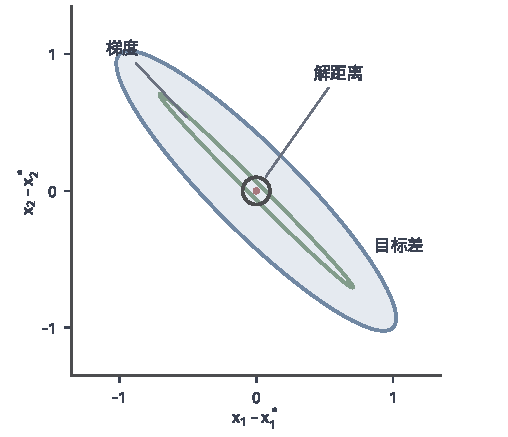
\includegraphics[width=86mm]{figures/05-optimization/01-linear-programming/matplotlib/opt-tolerance-regions/figure.pdf}
  \caption{同一个$\varepsilon=0.1$下三种指标的容差集合，横纵轴是相对于$\bm{x}^\star$的位移，目标取$\gamma=0.1$的拟合实例，$\bm{H}$的特征值为$0.1$和$2.1$。蓝色椭圆内目标差不超过$\varepsilon$，绿色椭圆内梯度大小不超过$\varepsilon$，深灰色小圆内解距离不超过$\varepsilon$。}
  \label{fig:opt-tolerance-regions}
\end{BookInlineFigure}

\paragraph{换算的条件：曲率的上下界}
前面的例子都指向曲率。把它变成定量结论，需要两个常数：曲率的下界$\mu$和上界$L$。全卷用$L$表示光滑常数，用$\kappa=L/\mu$表示条件数。这里先在二阶可微的情形下引入，用$\bm{A}\preceq\bm{B}$表示$\bm{B}-\bm{A}$半正定。第~\ref{chap:smooth-foundations}章将把$L$推广到只要求梯度Lipschitz连续的函数。

\begin{theorem}[三种误差的换算]
\label{thm:opt-error-conversions}
设$f:\mathbb{R}^n\to\mathbb{R}$二阶连续可微，且存在$0<\mu\leq L$，使对所有$\bm{x}$，
\begin{equation}
 \mu\bm{I}\preceq\nabla^2f(\bm{x})\preceq L\bm{I}.
 \label{eq:opt-curvature-bounds}
\end{equation}
则$f$有唯一最优解$\bm{x}^\star$，并且对任意$\bm{x}$，
\begin{equation}
 \begin{gathered}
 \frac{\mu}{2}e_d^2\leq e_f\leq\frac{L}{2}e_d^2,\qquad
 \mu e_d\leq e_g\leq Le_d,\\
 \frac{1}{2L}e_g^2\leq e_f\leq\frac{1}{2\mu}e_g^2.
 \end{gathered}
 \label{eq:opt-error-conversions}
\end{equation}
\end{theorem}

\begin{proof}
由定理~\ref{thm:opt-hessian-convex}，$f$是$\mu$强凸的，由第~\ref{sec:opt-optimality}节的结论，最优解存在且唯一。记$\bm{w}=\bm{x}-\bm{x}^\star$，$e_d=\lVert\bm{w}\rVert_2$。

第一组：由式~\eqref{eq:opt-taylor}，存在$s\in(0,1)$使
\[
 e_f=\frac12\bm{w}^\top\nabla^2f(\bm{x}^\star+s\bm{w})\bm{w}.
\]
再用式~\eqref{eq:opt-curvature-bounds}夹住二次型，即得。

第二组：由$\nabla f(\bm{x}^\star)=\bm{0}$和微积分基本定理，
\[
 \nabla f(\bm{x})=\bm{B}\bm{w},\qquad\bm{B}=\int_0^1\nabla^2f(\bm{x}^\star+s\bm{w})\,\mathrm{d}s.
\]
$\bm{B}$对称，其二次型是被积函数二次型的积分，所以特征值都在$[\mu,L]$内，于是
\[
 \mu\lVert\bm{w}\rVert_2\leq\lVert\bm{B}\bm{w}\rVert_2\leq L\lVert\bm{w}\rVert_2.
\]

第三组的右半：在式~\eqref{eq:opt-strong-support}中取$\bm{u}=\bm{x}$，右端是$\bm{v}$的二次函数，在$\bm{v}=\bm{x}-\nabla f(\bm{x})/\mu$处最小。所以对所有$\bm{v}$，
\[
 f(\bm{v})\geq f(\bm{x})-\frac{1}{2\mu}\lVert\nabla f(\bm{x})\rVert_2^2.
\]
取$\bm{v}=\bm{x}^\star$即得$e_f\leq e_g^2/(2\mu)$。

第三组的左半：由Taylor公式和$\nabla^2f\preceq L\bm{I}$，对任意$\bm{p}$有
\[
 f(\bm{x}+\bm{p})\leq f(\bm{x})+\langle\nabla f(\bm{x}),\bm{p}\rangle+\frac{L}{2}\lVert\bm{p}\rVert_2^2.
\]
取$\bm{p}=-\nabla f(\bm{x})/L$，得到
\[
 f^\star\leq f\Bigl(\bm{x}-\frac{1}{L}\nabla f(\bm{x})\Bigr)\leq f(\bm{x})-\frac{1}{2L}\lVert\nabla f(\bm{x})\rVert_2^2.
\]
移项即得$e_f\geq e_g^2/(2L)$。
\end{proof}

图~\ref{fig:opt-metric-conversions}把式~\eqref{eq:opt-error-conversions}画成一张换算图，每条箭头表示“已知箭尾的量，可以控制箭头的量”。凡用到$\mu$的箭头，都是从目标值或梯度推断位置，需要下弯曲率；用到$L$的箭头，是从位置推断目标值或梯度，需要上弯曲率有限。

\begin{BookInlineFigure}
  \centering
  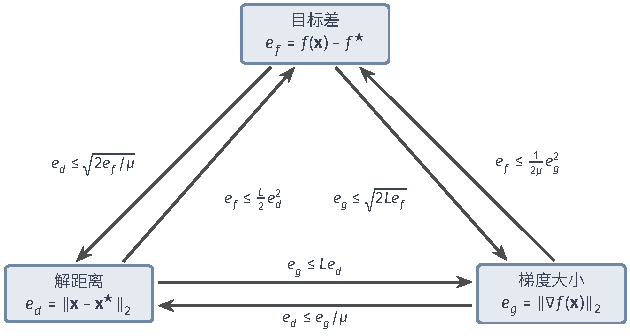
\includegraphics[width=106.74mm]{figures/05-optimization/01-linear-programming/tikz/opt-metric-conversions/figure.pdf}
  \caption{无约束时三种误差的换算，条件是$\mu\bm{I}\preceq\nabla^2f\preceq L\bm{I}$。箭头从已知量指向被控制的量。可计算的只有右下角的梯度大小，它指向其余两个量的两条箭头都依赖$\mu$。}
  \label{fig:opt-metric-conversions}
\end{BookInlineFigure}

用$\gamma=0.01$的实例代入。此时$\mu=0.01$，$L=2.01$，$\kappa=201$。对$\hat{\bm{x}}=(11,-9)$，右半边的两个上界是
\[
 e_f\leq\frac{e_g^2}{2\mu}\approx\frac{0.0202}{0.02}=1.01,\qquad
 e_d\leq\frac{e_g}{\mu}\approx14.2.
\]
实际值是$1.000$和$14.14$，两个界都很贴近，因为$\hat{\bm{x}}-\bm{x}^\star$几乎沿着平坦方向。而梯度约$0.142$这个数看起来很小，放大$1/\mu=100$倍后才是真实的距离。

两个常数不能互相替代，缺了一个，相应的箭头就断了。$\mu$接近零时，梯度几乎不提供关于目标差和距离的信息。$L$不存在时，距离小也不能保证梯度小：$\lvert x\rvert$在任意靠近$0$的点$x\neq0$处，梯度大小都是$1$。$\kappa$大表示两个方向的曲率差得远，同一个$e_d$对应的$e_g$可以相差$\kappa$倍。

\paragraph{有约束时：可行性}
定理~\ref{thm:opt-error-conversions}只针对无约束问题。有约束时，算法的输出可能不满足约束，目标差本身也就失去了意义。用\term{可行性残差}（feasibility residual）度量违反的程度：
\begin{equation}
 r_{\mathrm{feas}}(\hat{\bm{x}})=\max\Bigl\{\max_{i}\,\max\{g_i(\hat{\bm{x}}),0\},\ \max_{j}\,\lvert h_j(\hat{\bm{x}})\rvert\Bigr\}.
 \label{eq:opt-feasibility-residual}
\end{equation}
可行点的残差为零，残差大于零的点违反了至少一条约束。

资源分配中取点$\tilde{\bm{x}}=(2.1,2)$，它违反了两条资源约束：
\[
 g_1(\tilde{\bm{x}})=0.1,\qquad g_2(\tilde{\bm{x}})=0.2,\qquad r_{\mathrm{feas}}(\tilde{\bm{x}})=0.2.
\]
它的利润是$10.3$，比最优利润还高，也就是$f(\tilde{\bm{x}})-f^\star=-0.3<0$。多出来的利润并不是好事，它来自多用的资源。把两条约束相加的论证用在这里，利润至多超出$g_1+g_2=0.3$，恰好等于$0.3$。

反过来，可行点$(0,0)$的残差为零，利润却是$0$，目标差为$10$。图~\ref{fig:opt-feasibility-gap}中，绿点可行但利润不足，红叉利润过高但不可行。所以只报告目标值或只报告可行性都不够，两者要一起报告。

\begin{BookInlineFigure}
  \centering
  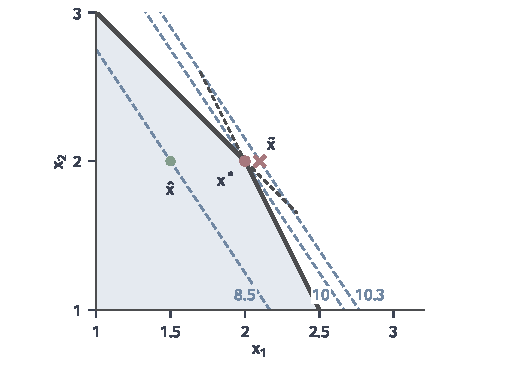
\includegraphics[width=88mm]{figures/05-optimization/01-linear-programming/matplotlib/opt-feasibility-gap/figure.pdf}
  \caption{目标值与可行性要一起看。浅蓝区域是资源分配的部分可行集，蓝色虚线旁的数字是利润。绿点$\hat{\bm{x}}=(1.5,2)$可行，利润$8.5$；红点$\bm{x}^\star=(2,2)$是最优解，利润$10$；红叉$\tilde{\bm{x}}=(2.1,2)$利润$10.3$，高于最优值，但违反了两条资源约束。}
  \label{fig:opt-feasibility-gap}
\end{BookInlineFigure}

约束的数值量纲也影响残差。把“工时”的单位换成分钟，同一条约束乘以$60$，残差也放大$60$倍，可行集却没有变。比较之前要先把约束的尺度说清楚。

\paragraph{有约束时：最优性残差}
第~\ref{sec:opt-optimality}节的图~\ref{fig:opt-boundary-directions}说明，有约束时梯度大小不再是合适的度量：最优解处的梯度不必为零。\term{最优性残差}（optimality residual）指这样一类量：在当前点可以计算，并且恰好在一阶条件成立时为零。无约束时它就是梯度大小。

一个能手算的情形是盒约束$\bm{C}=\{\bm{x}:l_i\leq x_i\leq u_i\}$，上下界允许取无穷。记$\Pi_{\bm{C}}$为逐坐标截断到$[l_i,u_i]$的投影，定义
\begin{equation}
 \bm{r}(\bm{x})=\bm{x}-\Pi_{\bm{C}}\bigl(\bm{x}-\nabla f(\bm{x})\bigr).
 \label{eq:opt-projected-residual}
\end{equation}
逐坐标看，记$g_i$为此处的第$i$个偏导数：$x_i$严格在区间内部时，$r_i=0$要求$g_i=0$；$x_i=l_i$时，$r_i=0$只要求$g_i\geq0$；$x_i=u_i$时，只要求$g_i\leq0$。这正是可行方向条件~\eqref{eq:opt-feasible-direction}逐坐标的写法。

取实例$\gamma=0.5$，加约束$x_1\geq1.2$。解在边界上：固定$x_1=1.2$，对$x_2$最小化得$x_2=8/15$，点$\bm{x}^\star=(1.2,8/15)$。此处的梯度由式~\eqref{eq:opt-ridge-gradient}算得
\[
 \nabla f(\bm{x}^\star)=\Bigl(\frac13,\ 0\Bigr).
\]
梯度不为零，但第一个坐标在下界上，偏导数非负，$\bm{r}(\bm{x}^\star)=\bm{0}$。这个问题是凸的，由上一节的充分性，$\bm{x}^\star$确实是最优解。

再看一个不是解的可行点$\hat{\bm{x}}=(1.5,0.5)$。此处$\nabla f(\hat{\bm{x}})=(0.75,0.25)$，先走一步再截断：
\[
 \hat{\bm{x}}-\nabla f(\hat{\bm{x}})=(0.75,0.25),\qquad
 \Pi_{\bm{C}}(0.75,0.25)=(1.2,0.25).
\]
所以$\bm{r}(\hat{\bm{x}})=(0.3,0.25)$，范数约为$0.39$。这个残差告诉我们，点还没有满足一阶条件。

一般约束的最优性残差要用到约束梯度的组合，由第~\ref{chap:constrained-optimality}章建立；非光滑目标没有梯度，相应的量由第~\ref{chap:nonsmooth-composite-optimization}章定义。这里只需记住它的职责：在不知道解的情况下，度量当前点离一阶条件还差多少。

\paragraph{精度标准}
表~\ref{tab:opt-metrics}汇总这些指标。后续各章陈述结果时，都要说清用的是哪一个。

\begin{table*}[!htbp]
  \centering
  \begin{tabular}{@{}llll@{}}
    \toprule
    指标 & 回答的问题 & 能否直接计算 & 换算所需条件\\
    \midrule
    目标差$e_f$ & 结果比最好差多少 & 需要$f^\star$或其下界 & 可行点；$\mu$可换成距离，$L$可换成梯度\\
    解距离$e_d$ & 位置差多远 & 需要解集 & 解不唯一时参照解集；$L$可换成目标差和梯度\\
    梯度大小$e_g$ & 局部还有多少下降余地 & 能 & 无约束；$\mu$才能换成目标差和距离\\
    可行性残差$r_{\mathrm{feas}}$ & 违反约束多少 & 能 & 依赖约束的尺度\\
    最优性残差 & 离一阶条件还差多少 & 能 & 凸问题中才对应全局最优\\
    \bottomrule
  \end{tabular}
  \caption{近似解的评价指标。前三项针对无约束或已知可行的点，后两项用于约束问题；换算条件的含义见定理~\ref{thm:opt-error-conversions}。}
  \label{tab:opt-metrics}
\end{table*}

阈值的取法也要交代。绝对标准$e_g\leq\varepsilon$依赖目标的尺度：把$f$整体乘以$100$，解不变，梯度却放大$100$倍，同一个$\varepsilon$的严格程度就变了。所以实践中常用相对标准，例如
\begin{equation}
 \lVert\bm{g}^{(t)}\rVert_2\leq\varepsilon\,\max\bigl\{1,\lVert\bm{g}^{(0)}\rVert_2\bigr\}.
 \label{eq:opt-relative-stopping}
\end{equation}

评价方法与决定停止是两种场合。比较方法时，常对同一问题先用高精度方法算出参照值$f^\star$，再看目标差随计算量的变化；参照值本身也有误差，应当说明怎样得到。实际求解时$f^\star$未知，只能依据可计算的残差决定何时停止，而残差小对目标差意味着什么，取决于$\mu$这样的条件。

最后要区分算法的结论。说“迭代收敛到驻点”“输出满足$e_g\leq\varepsilon$”“输出是$\varepsilon$最优解”，是三个强度依次上升的陈述，中间隔着凸性或曲率下界这样的条件。迭代次数与每步代价怎样计入比较，由第~\ref{chap:smooth-foundations}章规定。
